\subsection{Mesh Representation and Reconstruction}
\label{ch3:sec:reconstruction}
In this experiment, we evaluate the quality of our mesh representations.
We encode multiple airfoils into latent codes using Eq.\ref{ch3:eq:autodec}.
No manual adjustments are required when working with different airfoils.
The embedding quality is measured by the accuracy of surface reconstruction decoded from the latent codes.

\begin{figure}[th]
	\begin{center}
		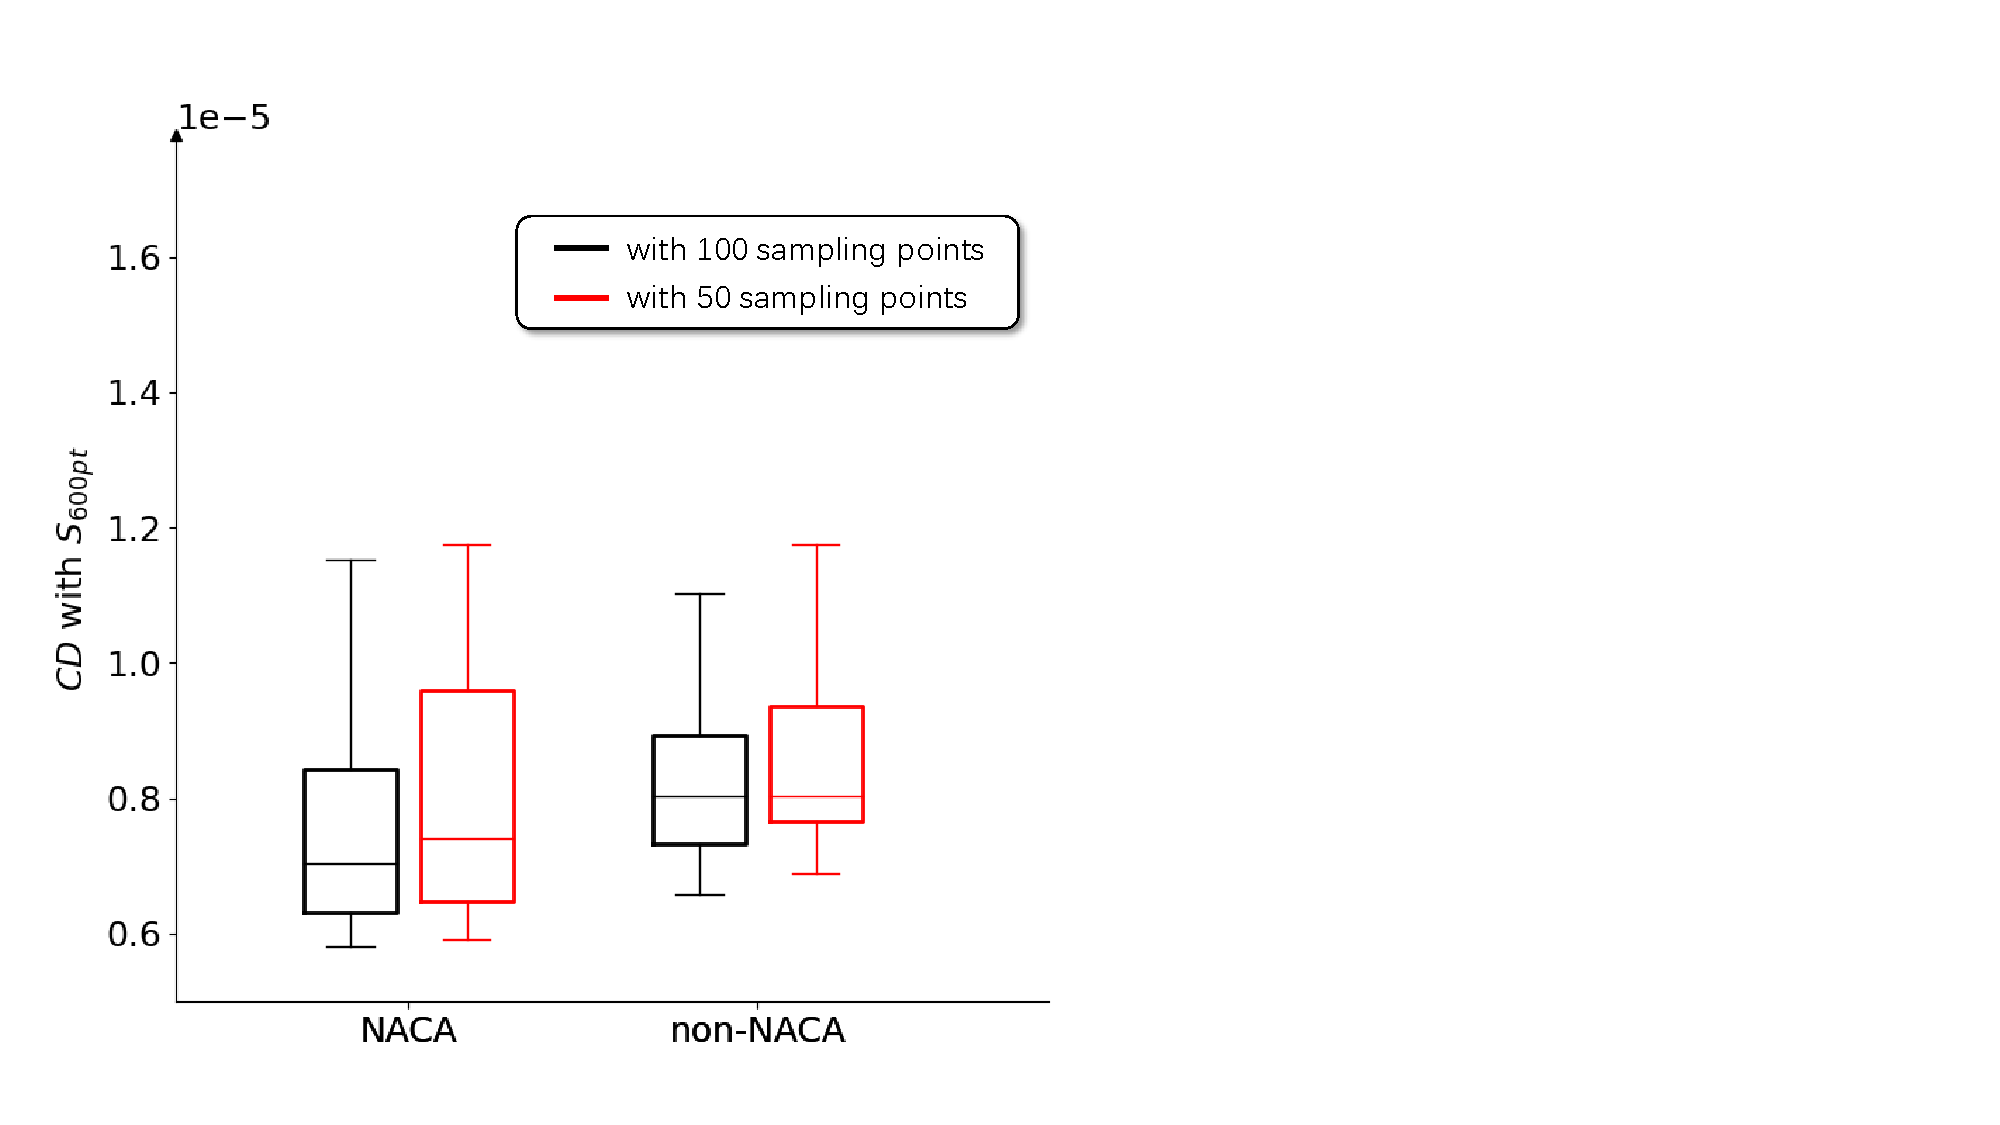
\includegraphics[width=0.5\linewidth]{chapter3/tex/figures/experiment/reconstruction_evaluation.pdf}
	\end{center}
	\caption{
		\small The \textit{Chamfer Distance} (CD) between the reconstructed airfoils and the 600-point reference geometries.
		%NACA and non-NACA airfoils are tested, with 100-point and 50-point geometries as the reconstruction targets.
	}
	\label{ch3:fig:exp_recon_eval}
\end{figure}

To do this, we randomly chose 50 NACA airfoils outside the training set.
We also use another 50 non-NACA airfoils, to investigate the model's generalization ability.
These non-NACA airfoils belongs to the AG and RG series, plus the low-Reynolds-number Eppler airfoils, which are collected from the UIUC airfoil dataset \cite{aa.Selig1996}.
Since most airfoil geometric data publicly available samples a surface with 50 to 100 points, we sample 100 and 50 surface points on each airfoil as the target geometries to test  under different sampling qualities.
We use 600 sampling points $S_{600pt}$ on an airfoil as a lossless geometry.
The reconstruction error is calculated by the Chamfer Distance \cite{ai.Barrow1977} ($CD$) between the deformed airfoil surface and  $S_{600pt}$, which is defined as
\begin{equation}
    CD({V^S},{S_{600pt}}) = \frac{1}{{|{V^S}|}}\sum\limits_{{v_i} \in {V^S}} {\mathop {\min }\limits_{{s_i} \in {S_{600pt}}} ||{v_i} - {s_i}|{|^2}}  + \frac{1}{{|{S_{600pt}}|}}\sum\limits_{{s_i} \in {S_{600pt}}} {\mathop {\min }\limits_{{v_i} \in {V^S}} ||{v_i} - {s_i}|{|^2}} \,.
\end{equation}
Since $V^S$ and $S_{600pt}$ are discrete sampling of a continuous airfoil profile, $CD$ remains positive even when two shapes are exactly registered.

\begin{figure}[!htb]
	\begin{center}
		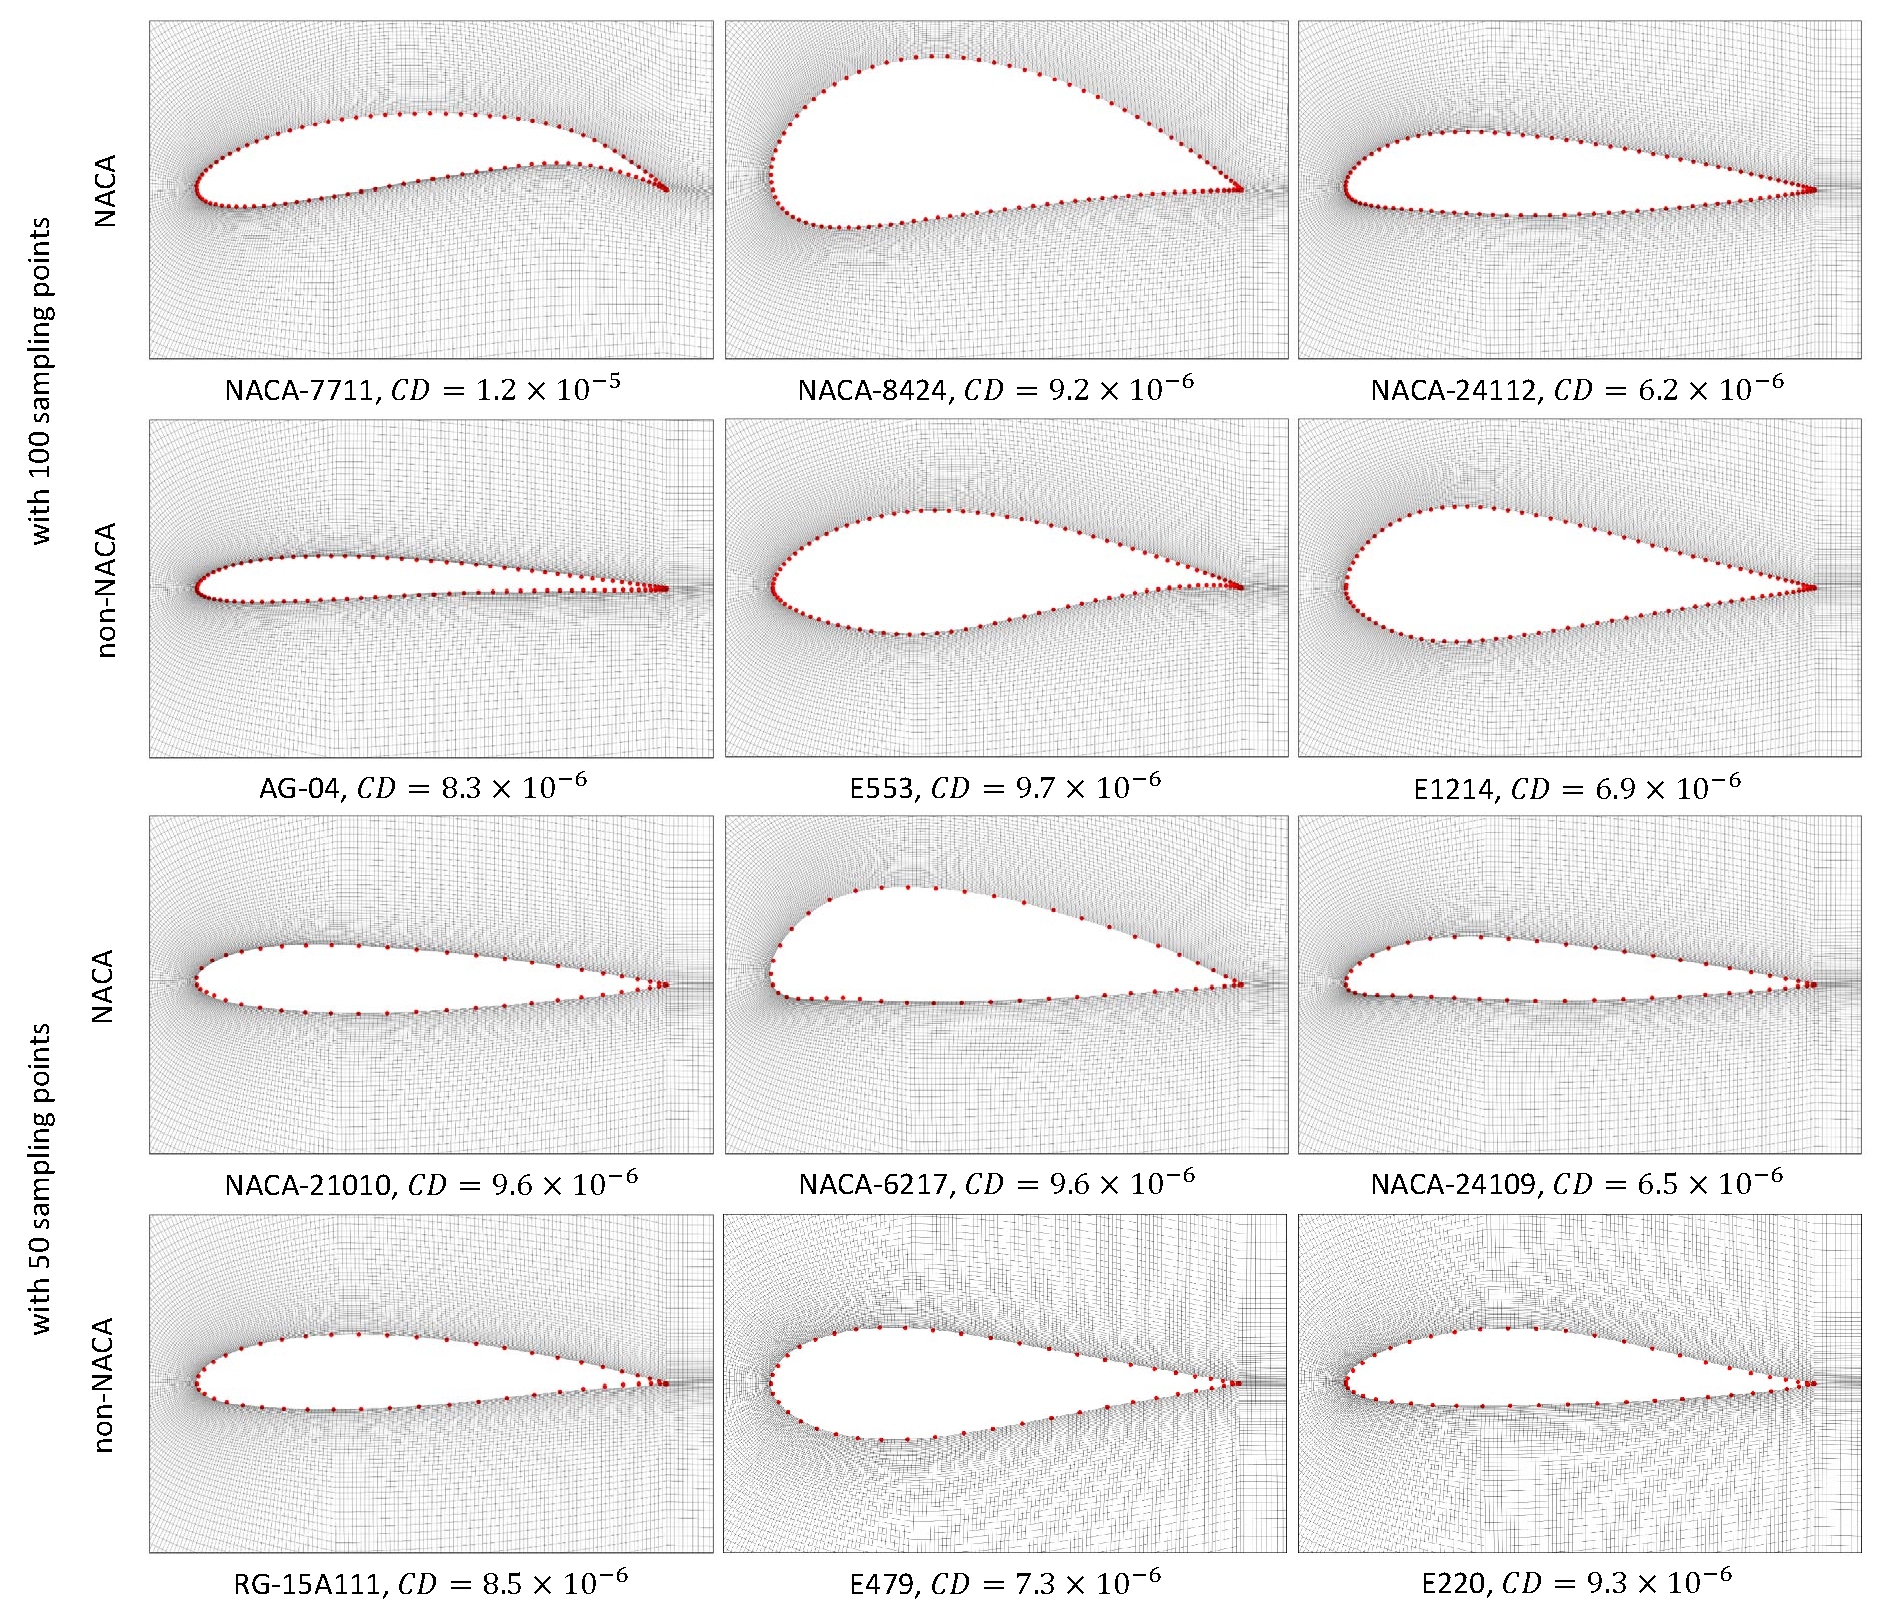
\includegraphics[width=1\linewidth]{chapter3/tex/figures/experiment/reconstruction_result.pdf}
	\end{center}
	\caption{
		\small The reconstructions of various airfoil series with different numbers of sampled points, i.e. the red dots.
		$CD$s are shown.
	}
	\label{ch3:fig:exp_recon_res}
\end{figure}

Fig.\ref{ch3:fig:exp_recon_eval} shows the reconstruction accuracy over the 50 test airfoils.
The mean $CD$s are $8.9\times 10^{-6}$ and $9.3\times 10^{-6}$ for 100-point and 50-point $S$ over NACA airfoils, and those are $8.3\times 10^{-6}$ and $8.7\times 10^{-6}$ for non-NACA airfoils. The errors are very small. 
We visualize some reconstruction results in Fig.\ref{ch3:fig:exp_recon_res}.
The figure shows that the reported mean $CD$s indicate high-fidelity reconstructions of both airfoil types and under both sampling qualities.
At the same time, the statistics and the qualitative results show little performances difference between NACA and non-NACA airfoils.
The proposed model can work well with other shapes that are similar to the training geometries without additional adaptations.
For all test settings, the average time cost to encode and reconstruct a given airfoil is $30.1s$ on a standard PC with an NVIDIA V100 GPU card.